\documentclass[11pt]{article}

\usepackage[utf8]{inputenc}
\usepackage[T1]{fontenc}
\usepackage{graphicx}
\usepackage[linktocpage=true]{hyperref}
\usepackage{todonotes}
\usepackage{mathpazo}
\usepackage[english]{babel}
\usepackage[skins]{tcolorbox}
\usepackage{csquotes}
\usepackage{rotating}
\usepackage{hyperref}
\usepackage{multicol}
\usepackage{courier}

\hypersetup{
    colorlinks=true,
    linkcolor=blue,
    filecolor=magenta,      
    urlcolor=blue,
    citecolor=black
}

\usepackage[
backend=biber,
style=alphabetic,
sorting=ynt
]{biblatex}
\addbibresource{myBibliography.bib}

\newcommand{\projectName}{Contract Instruction Application}

\begin{document}
\begin{titlepage}
	\newcommand{\HRule}{\rule{\linewidth}{0.5mm}}
    \begin{center}
    
    	\HRule\\[0.4cm]
    	
    	{\huge\bfseries Contract Instruction Application}\\[0.2cm]
    	
    	{\huge User Manual}\\[0.2cm]

    	\HRule\\[0.5cm]

	    \textsc{\textbf{Kyle Gaunt} - u15330967}\\[0cm]
	    \textit{BScIT IKS (UP)}\\[0.5cm]
        \includegraphics[scale=0.3]{images/ApplicationLogos/CI_Logo.png}
    
    \end{center}
\end{titlepage}
\tableofcontents
\newpage

\section{Introduction}
\begin{center}
\begin{tcolorbox}[skin=widget,
boxrule=1mm,
coltitle=black,
colframe=blue!45!white,
colback=blue!15!white,
width=(.9\linewidth),before=\hfill,after=\hfill,
adjusted title={CONTRACT INSTRUCTION}]
\textit{A written instruction issued by or under the authority of the principal agent to the contractor, which may include drawings and other construction information.}
\tcblower
\cite{ciDefinition}
\end{tcolorbox}
\end{center}
\begin{flushleft}
The Contract Instruction Application is for the professional construction worker who wants to leave outdated processes in the past, by using innovative software that solves all the problems of pen to paper administration quickly and effectively so that more time can be spent focusing on what needs to be done and how.\\[0.5cm]

The application has been designed to allow users to issue, edit and interact with CIs while on site or in the comfort of their workplace or (especially during Covid times) home office. The system design allows for availability and accessibility, for users at any given time in order to fit in with the ever changing schedules that the construction industry is known for.\\[0.5cm]
Users are able to use the most innovative CI system that boasts a large variety of functionality, that allows the users to:\\[0.5cm]
\begin{itemize}
    \item Create CIs that include any important information such as what is being instructed and why
    \item Specify the individual components within the project that will be affected by the CI being issued
    \item Attach any relevant files in the form of images, PDFs or any other file types that are required
    \item Include any professionals that are involved in the project
\end{itemize}
The system provides users with secure login and a variety of security features that ensure all information relating to the CIs (and by extension the companies that they represent) is kept safe and secure.\\[0.5cm]

Users have total control and are able to manage all components of their own profile, including:
\begin{itemize}
    \item Profile picture
    \item First and Last names
    \item Contact details
    \item Password
\end{itemize}

Users can access and edit all of their CIs at any time of the day and all changes made will be instantaneously shared across all users involved in the project.\\[0.5cm]

This document will explain how the system has been deployed as well as guide the user through the various use cases that the user will encounter when using the CI application.\\[0.5cm]
\end{flushleft}

\newpage

\section{Deployment Diagram}
    \subsection{Description}
    The system is designed using a 3-tier architecture pattern which means that each subsystem is capable of being self-sufficient and not reliant on any other subsystem. To achieve this, the system has been designed with low coupling and high cohesion in mind.\\[0.5cm]
    Two user interfaces (Presentation tier) are supported (Android and web browser compatible version) which both communicate with the database independently of one another. All database queries are performed using TCP/IP protocol. This protocol is preferable to UDP as the information needs to be secure and accurate for all users on the system.\\[0.5cm]
    The database (Data tier) makes use of an Interpreter pattern to make queries to the mySQL database that is supported by Heroku (the cloud based hosting service).\\[0.5cm]
    Finally, the Application tier is responsible for communicating with the resource manager to request more or less resources according to the current system load.\\[0.5cm]
    \subsection{Software Logos}
    For your convenience, enlarged versions of software logos:\\[0.5cm]
    Android:\\[0.5cm]
    
\includegraphics[width=20pt]{images/ApplicationLogos/Android.png}
    \newline
    Chrome Web Browser:\\[0.5cm]
    
\includegraphics[width=20pt]{images/ApplicationLogos/Chrome.png}
    \newline
    Docker:\\[0.5cm]
    
\includegraphics[width=30pt]{images/ApplicationLogos/Docker.png}
    \newline
    Heroku:\\[0.5cm]
    
\includegraphics[width=40pt]{images/ApplicationLogos/Heroku.png}
    \newline
    Kubernetes:\\[0.5cm]
    
\includegraphics[width=50pt]{images/ApplicationLogos/Kubernetes.png}
    \newline
    \subsection{Diagram}
    \textit{Please see the diagram below.}\\[0.5cm]
    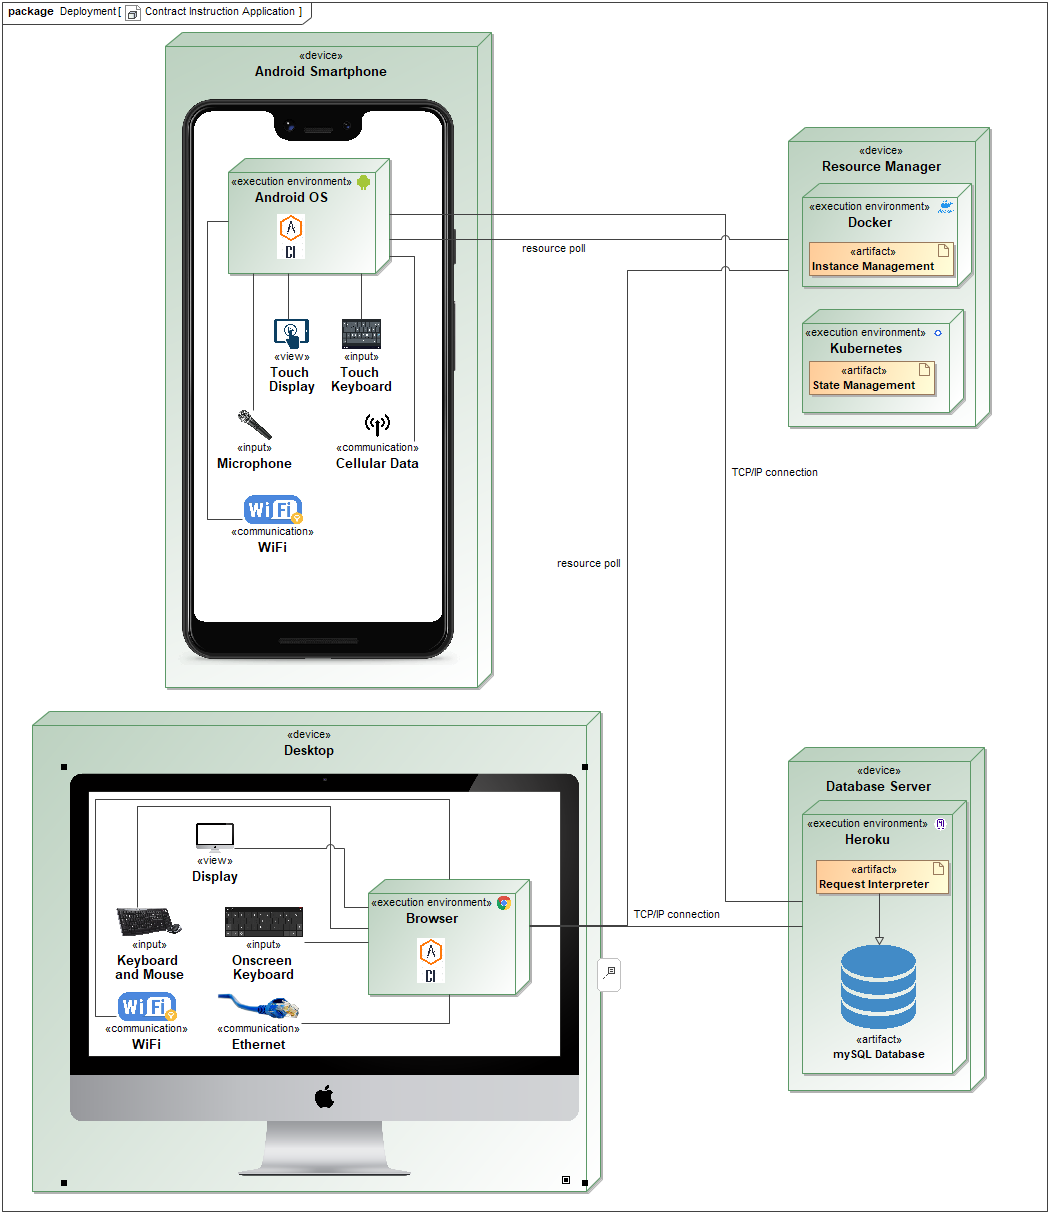
\includegraphics[scale=0.5]{images/DeploymentModel.PNG}
\newpage

\section{How to Use the CI Application}
    \subsection{\textit{Use Case 1} - \uppercase{Create a New Contract Instruction}}
        \textit{Step 1 -} On the \textit{Home} screen, press the "New Contract Instruction" button. You will be directed to the \textit{Create New CI} screen.\\[0.5cm]
        \begin{center}
            \includegraphics[scale=0.3]{images/UseCase1/HomePage_1.PNG}
        \end{center}
        \textit{Step 2:}\\[0.5cm]
        \textit{Step 2.1 -} The new CI will automatically be numbered as: \newline
        \begin{center}
            \texttt{number of the most recent CI + 1}.\\[0.5cm]
        \end{center}
        \textit{Step 2.2 -} Specify the name of the new CI.\\[0.5cm]
        \begin{center}
            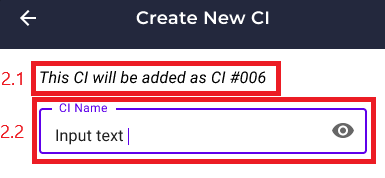
\includegraphics[scale=0.5]{images/UseCase1/NewCIPage_1-1.png}
        \end{center}
        \textit{Step 3:}\\[0.5cm]
        \textit{Step 3.1 -} Press the "Select Recipients" drop down menu. The drop down will display all professionals that can be included in the CI.\\[0.5cm]
        \begin{center}
            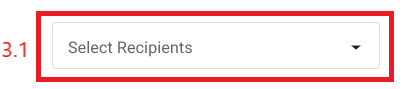
\includegraphics[scale=0.5]{images/UseCase1/NewCIPage_1-2.png}
        \end{center}
        \textit{Step 3.2 -} Select all professionals to add to the CI using the check boxes in the drop down menu.\\[0.5cm]
        \begin{center}
            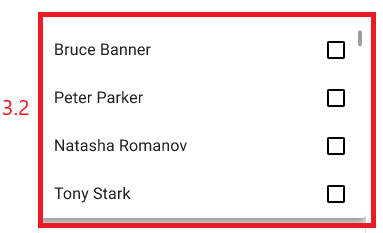
\includegraphics[scale=0.5]{images/UseCase1/NewCIPage_2-1.png}
            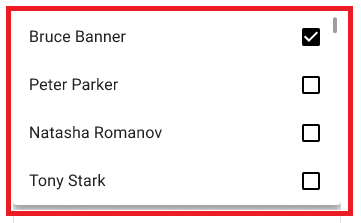
\includegraphics[scale=0.5]{images/UseCase1/NewCIPage_2-2.png}
        \end{center}
        \textit{Step 4 -} Enter the relevant information into the "Description" field. This field can be left blank.\\[0.5cm]
        \begin{center}
            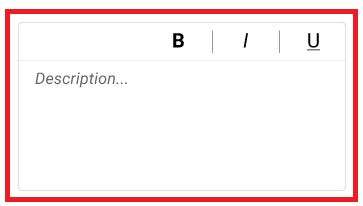
\includegraphics[scale=0.5]{images/UseCase1/NewCIPage_1-3.png}
        \end{center}
        \textit{Step 5 -} Enter the relevant information into the "Reason for Change" field. This field can be left blank.\\[0.5cm]
        \begin{center}
            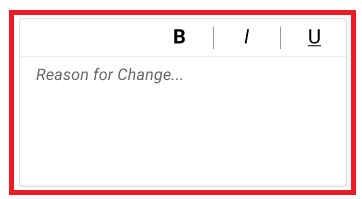
\includegraphics[scale=0.5]{images/UseCase1/NewCIPage_1-4.png}
        \end{center}
        \textit{Step 6 -} Select the applicable areas that will be affected by the CI. The user can select zero to four options, depending on their requirements.\\[0.5cm]
        \begin{center}
            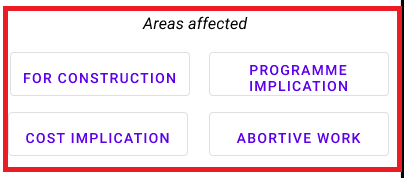
\includegraphics[scale=0.5]{images/UseCase1/NewCIPage_4-1.png}
            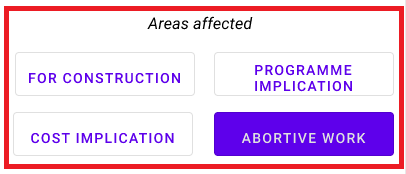
\includegraphics[scale=0.5]{images/UseCase1/NewCIPage_4-2.png}
        \end{center}
        \textit{Step 7 -} Upload any files that need to be included in the CI. This can be done via the device's on board memory, built in camera or a cloud-based storage service. The uploaded files will be displayed below the upload buttons.\\[0.5cm]
        \begin{center}
            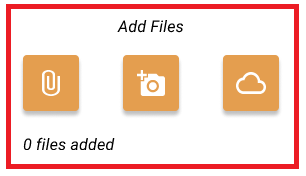
\includegraphics[scale=0.5]{images/UseCase1/NewCIPage_5-1.png}
            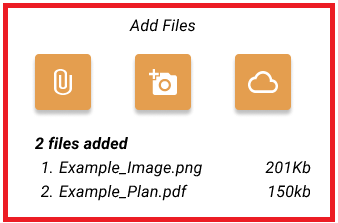
\includegraphics[scale=0.5]{images/UseCase1/NewCIPage_5-2.png}
        \end{center}
        \textit{Step 8 -} Press the "Submit" button to create the new CI. A Toast Notification will be displayed at the bottom of the screen to confirm the creation of the CI.\\[0.5cm]
        \begin{center}
            
\includegraphics[scale=0.5]{images/UseCase1/NewCIPage_6-1.png}
            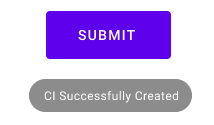
\includegraphics[scale=0.5]{images/UseCase1/NewCIPage_6-2.PNG}
        \end{center}
    \subsection{\textit{Use Case 2} - \uppercase{View a Contract Instruction}}
            \textit{Step 1 -} From the \textit{Home} page, select a CI from the list of "Existing Contract Instructions" by tapping on the CI card that you want to open. The user can make use of the "Filter" button to refine their search.\\[0.5cm]
            \begin{center}
                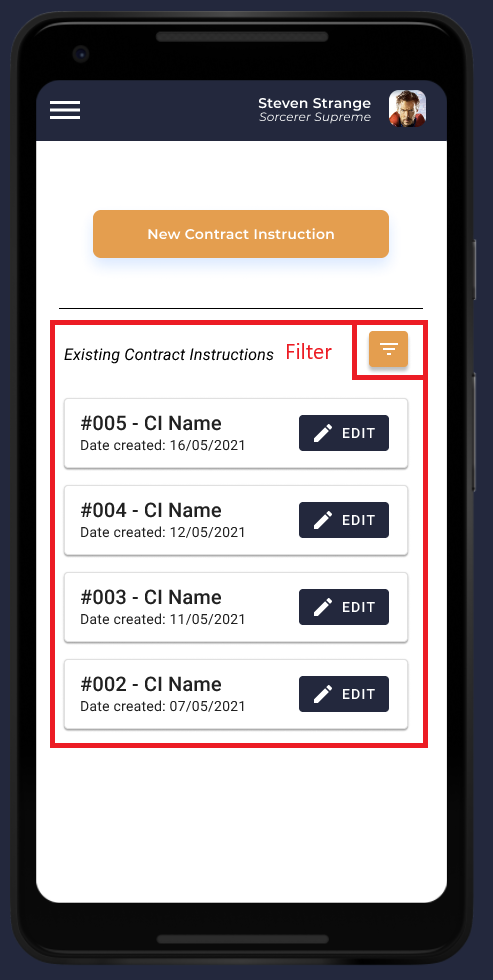
\includegraphics[scale=0.5]{images/UseCase2/HomePage_1-1.png}
            \end{center}
            \textit{Step2 - } You will be directed to the \textit{View CI} page where you will be able to see the details of the CI you selected.\\[0.5cm]
            \begin{center}
                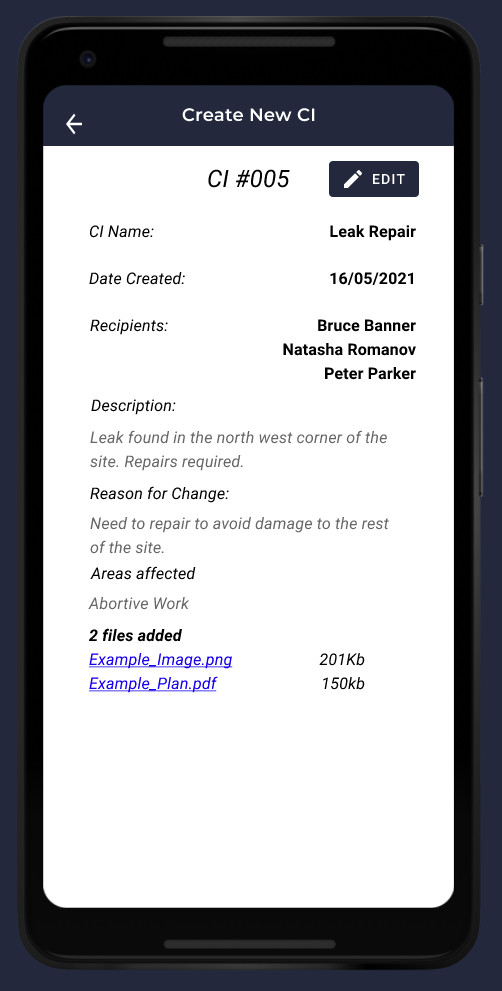
\includegraphics[scale=0.5]{images/UseCase2/ViewCIPage_1.PNG}
            \end{center}
    \subsection{\textit{Use Case 3} - \uppercase{Edit a Contract Instruction}}
            \textit{Step 1 -} From the \textit{Home} page, select a CI to edit from the list of "Existing Contract Instructions" by tapping on the edit button on the card of the CI that you want to open. The user can make use of the "Filter" button to refine their search. The user will be directed to the \textit{Edit CI Page}.\\[0.5cm]
            \begin{center}
                \includegraphics[scale=0.5]{images/UseCase3/HomePage_1.png}
            \end{center}
            \textit{Step 2:}\\[0.5cm]
            \textit{Step 2.1 - 2.4:} Alter any information within the CI as needed. The CI number cannot be changed (for official purposes).\\[0.5cm]
            \begin{center}
                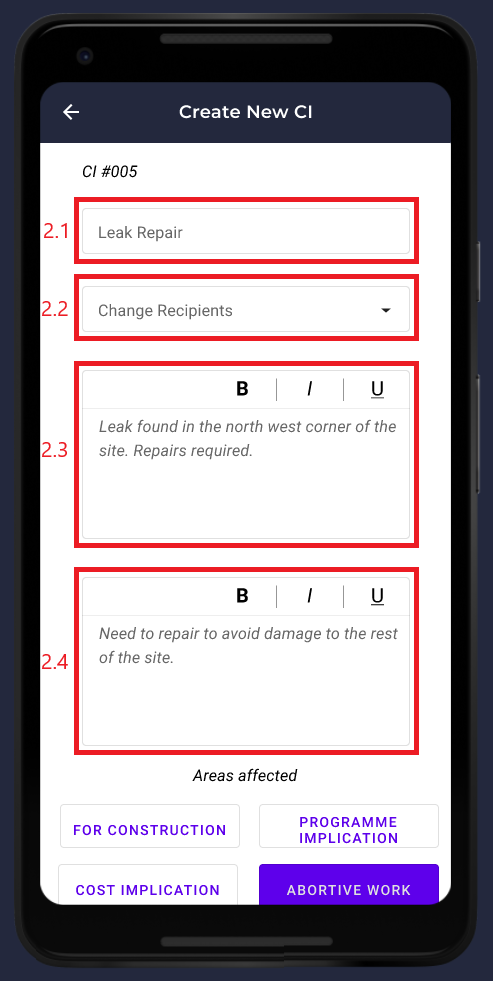
\includegraphics[scale=0.5]{images/UseCase3/EditCI_1-3.png}
            \end{center}
            \textit{Step 2.5 -} Add/remove areas affected by selecting/deselecting the specific area.\\[0.5cm]
            \textit{Step 2.6 -} Add new images to the CI by selecting a method of attaching under the "Add Files" section.\\[0.5cm]
            \textit{Step 2.7 -} Remove images by tapping the "X" button next to the image.\\[0.5cm]
            \textit{Step 2.8 -} Tap the "Update" button to commit the changes. \\[0.5cm]
            \begin{center}
                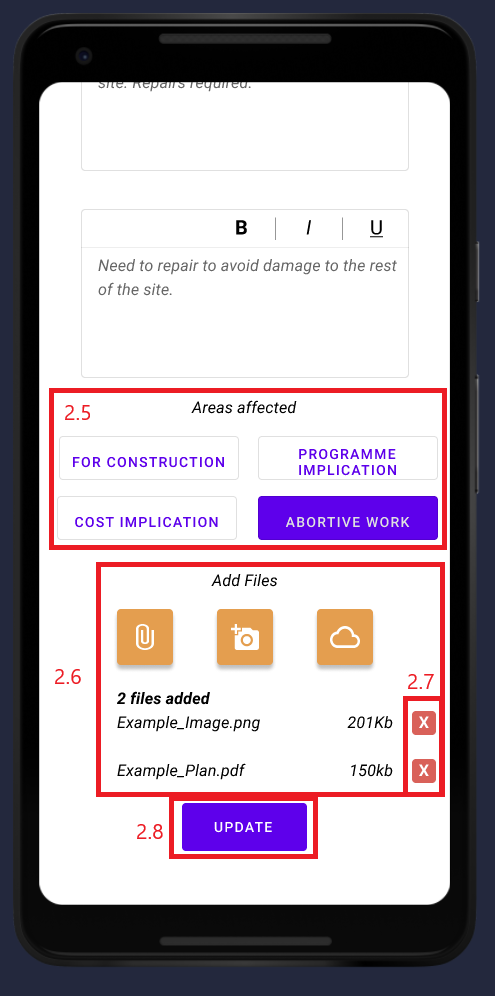
\includegraphics[scale=0.5]{images/UseCase3/EditCI_1-4.png}
            \end{center}
            \textit{Step 2.9 -} A Toast Notification will be displayed at the bottom of the screen to confirm that the updates have been made to the CI.\\[0.5cm]
            \begin{center}
                
\includegraphics[scale=0.5]{images/UseCase3/EditCI_1-5.PNG}
            \end{center}
    \subsection{\textit{Use Case 4} - \uppercase{User Management}}
        \subsubsection{\textit{Use Case 4.1} - \uppercase{Sign In}}
            \textit{Step 1:}\\[0.5cm]
            \textit{Step 1.1:} Enter email address into the "Email Address" field.\\[0.5cm]
            \textit{Step 1.2:} Enter password into "Password" field.\\[0.5cm]
            \textit{Step 1.3:} Press the "Sign In" button to sign in to the CI Application. If successful, the user will be directed to the \textit{Home} page. If not, the user will be asked to reenter the email address and password.\\[0.5cm]
            \begin{center}
                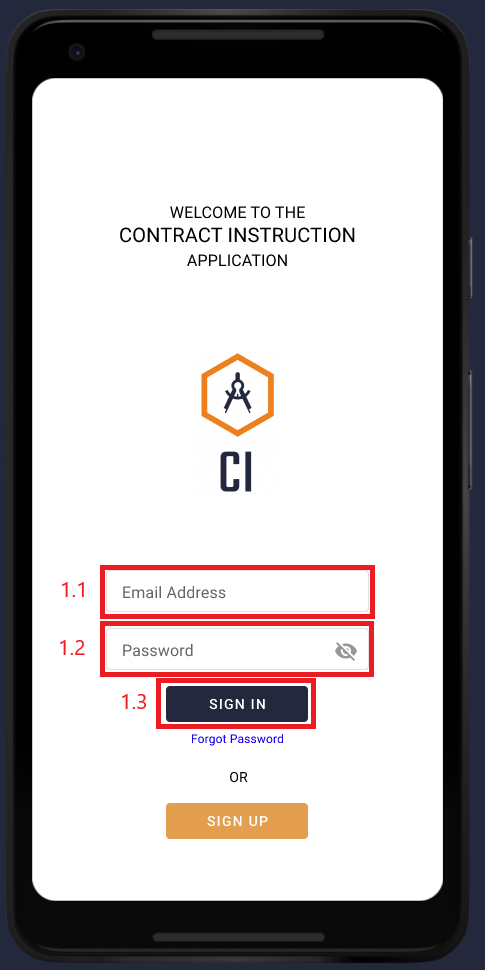
\includegraphics[scale=0.5]{images/UseCase4/SignInPage_1-1.png}
            \end{center}
        \subsubsection{\textit{Use Case 4.2} - \uppercase{View Your Profile}}
            \textit{Step 1 -} On the \textit{Home} page, expand the navigation drawer by tapping the 3 line button in the top left of the screen.\\[0.5cm]
            \begin{center}
                \includegraphics[scale=0.5]{images/UseCase4/HomePage_1.PNG}
            \end{center}
            \textit{Step 2 -} After the navigation drawer slides out, tap on the "My Profile" button. The user will be directed to the \textit{My Profile} page.\\[0.5cm]
            \begin{center}
                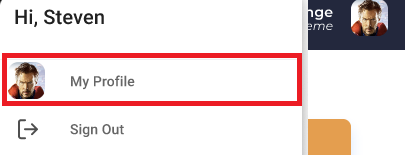
\includegraphics[scale=0.5]{images/UseCase4/MyProfilePage_1-1.png}
                \newline
                \newline
                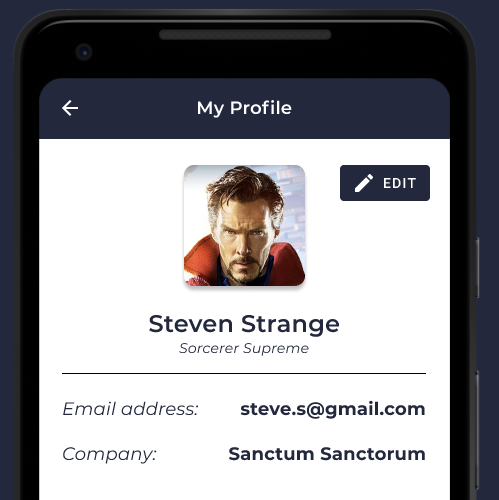
\includegraphics[scale=0.5]{images/UseCase4/MyProfilePage_1-2.png}
            \end{center}
        \subsubsection{\textit{Use Case 4.3} - \uppercase{Edit Your Profile}}
            \textit{Step 1 -} On the \textit{Home} page, expand the navigation drawer by tapping the 3 line button in the top left of the screen.\\[0.5cm]
            \begin{center}
                \includegraphics[scale=0.5]{images/UseCase4/HomePage_1.PNG}
            \end{center}
            \textit{Step 2 -} After the navigation drawer slides out, tap on the "My Profile" button. The user will be directed to the \textit{My Profile} page.\\[0.5cm]
            \begin{center}
                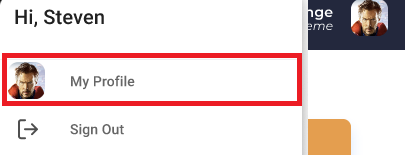
\includegraphics[scale=0.5]{images/UseCase4/MyProfilePage_1-1.png}
                \newline
                \newline
                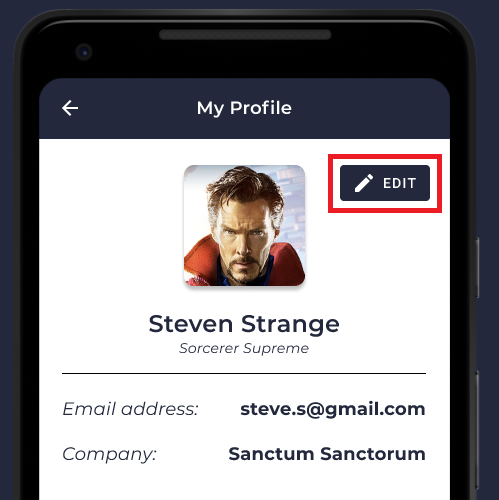
\includegraphics[scale=0.5]{images/UseCase4/MyProfilePage_1-3.png}
            \end{center}
            \textit{Step 3 -} Tap the "Edit" button. The user will be directed to the \textit{Edit Profile} page.\\[0.5cm]
            \textit{Step 4:}\\[0.5cm]
            \textit{Step 4.1 - 4.6:} Alter any information within the user profile as required, including profile picture, first name, last name, email address, company and password.\\[0.5cm]
            \textit{Step 4.7 -} Tap the "Update" button to commit the changes.\\[0.5cm]
            \begin{center}
                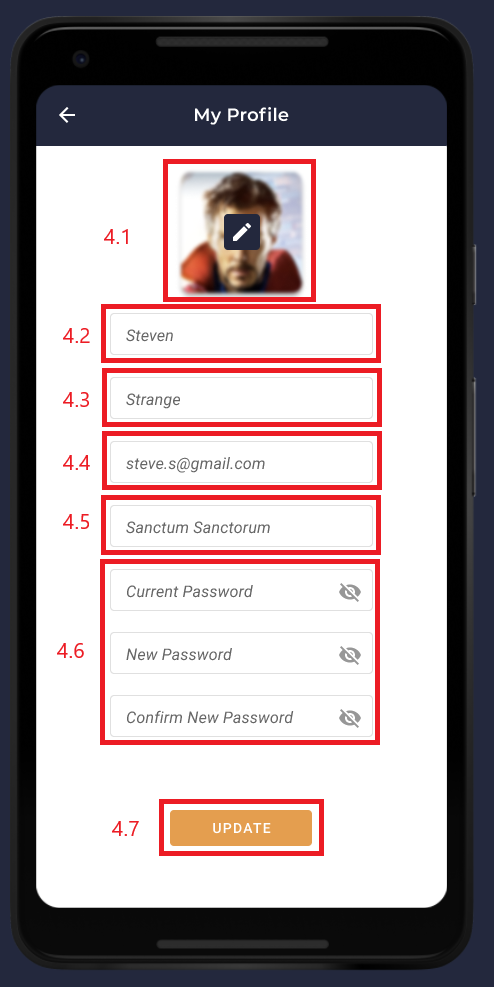
\includegraphics[scale=0.5]{images/UseCase4/EditProfile_1-2.png}
            \end{center}
        \subsubsection{\textit{Use Case 4.4} - \uppercase{Sign Out}}
            \textit{Step 1 -} On the \textit{Home} page, expand the navigation drawer by tapping the 3 line button in the top left of the screen.\\[0.5cm]
            \begin{center}
                \includegraphics[scale=0.5]{images/UseCase4/HomePage_1.PNG}
            \end{center}
            \textit{Step 2 -} After the navigation drawer slides out, tap on the "Sign Out" button. The user will be signed out and directed to the \textit{Sign In} page.\\[0.5cm]
            \begin{center}
                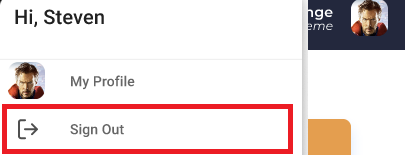
\includegraphics[scale=0.5]{images/UseCase4/SignOut_1-2.png}
            \end{center}
        \subsubsection{\textit{Use Case 4.5} - \uppercase{Sign Up}}
            \textit{Step 1:} Press the "Sign Up" button to create a CI Application account. The user will be directed to the \textit{Sign Up} page.\\[0.5cm]
            \begin{center}
                \includegraphics[scale=0.5]{images/UseCase4/SignInPage_1-2.png}
            \end{center}
            \textit{Step 2:}\\[0.5cm]
            \textit{Step 2.1 -} Enter first name in the "First Name" field. This field is mandatory.\\[0.5cm]
            \textit{Step 2.2 -} Enter last name in the "Last Name" field. This field is mandatory.\\[0.5cm]
            \textit{Step 2.3 -} Enter email address in the "Email Address" field. This field is mandatory.\\[0.5cm]
            \textit{Step 2.4 -} Enter company name in the "Company" field.\\[0.5cm]
            \textit{Step 2.5 -} Enter password in the "Password" field. This field is mandatory.\\[0.5cm]
            \textit{Step 2.6 -} Confirm password in the "Confirm Password" field. This field's input must \textbf{exactly} match the input of 2.5. This field is mandatory.\\[0.5cm]
            \textit{Step 2.7 -} Confirm the sign up process by pressing the "Sign Up" button. The user will be directed back to the \textit{Sign In} page where they can now sign in to the CI Application.\\[0.5cm]
            \begin{center}
                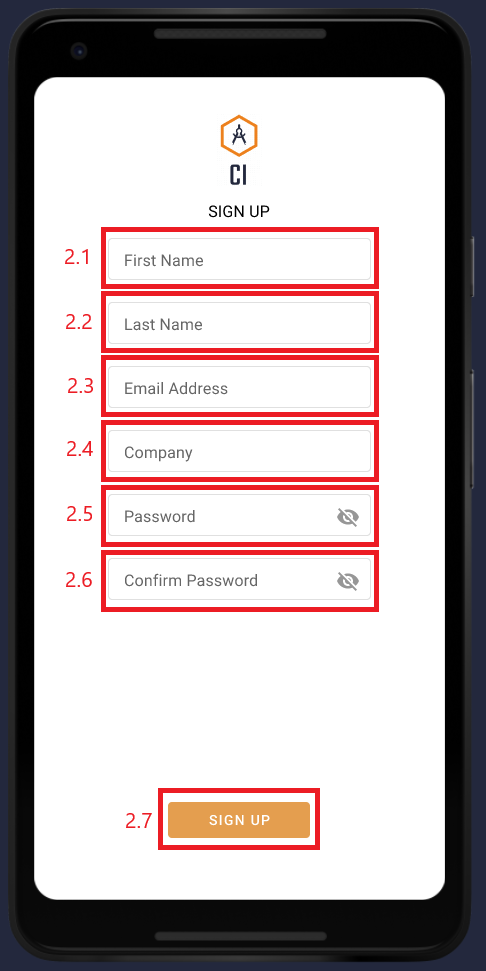
\includegraphics[scale=0.5]{images/UseCase4/SignUpPage.PNG}
            \end{center}
        \subsubsection{\textit{Use Case 4.6} - \uppercase{Reset Password}}
        \textit{Step 1 -} On the \textit{Sign Up} page, press the "Forgot Password" link. The user will be redirected to the \textit{Password Reset} page.\\[0.5cm]
        \begin{center}
            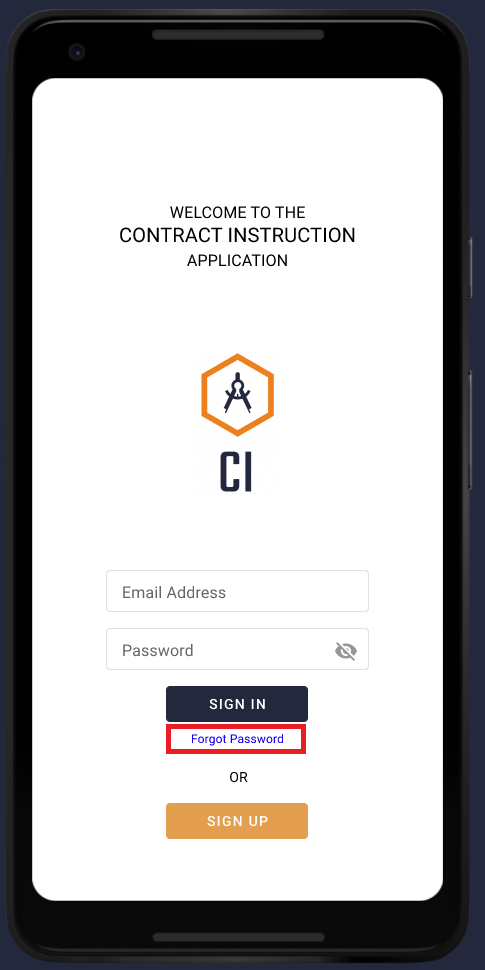
\includegraphics[scale=0.5]{images/UseCase4/SignInPage_1-3.png}
        \end{center}
        \textit{Step 2 -} Enter email address associated with the account.\\[0.5cm]
        \begin{center}
            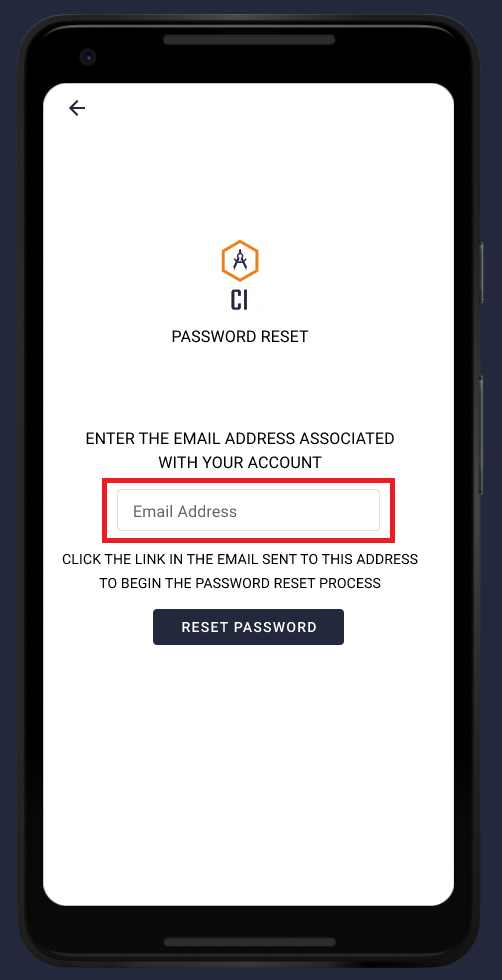
\includegraphics[scale=0.5]{images/UseCase4/ResetPassword_1-2.png}
        \end{center}
        \textit{Step 3:}
        \textit{Step 3.1 -} Press the "Reset Password" button.\\[0.5cm]
        \begin{center}
            
\includegraphics[scale=0.5]{images/UseCase4/ResetPassword_1-3.png}
        \end{center}
        \textit{Step 3.2 -} A Toast Notification will be displayed at the bottom of the screen to confirm password reset email has been sent.\\[0.5cm]
        \begin{center}
            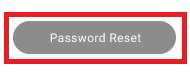
\includegraphics[scale=0.5]{images/UseCase4/PasswordResetToast_1-1.PNG}
        \end{center}
\end{document}
